\subsection{Space Shift Keying Modulation
}

How can the actors communicate, if the result is a diagonal matrix with random value?

We will use a technique called \textit{Space Shift Keying} (SSK) Modulation \cite{5165332}, where \textit{antenna indices are used as the only means to relay information}. Given $K$ the number of antenna of the actors in the system, we can send $log_2(K)$ bits by mapping each combination of bits to a specific antenna.
\footnote{This may seem rather unoptimized, as we use only one antenna instead of combinations of them. To see a more general approach, the authors also wrote the paper \cite{4699782}, where they discuss a more general approach using multiple active antennas at the same time. The general approach will also work with our proposed solution.}

\begin{figure}[H]
  \centering
  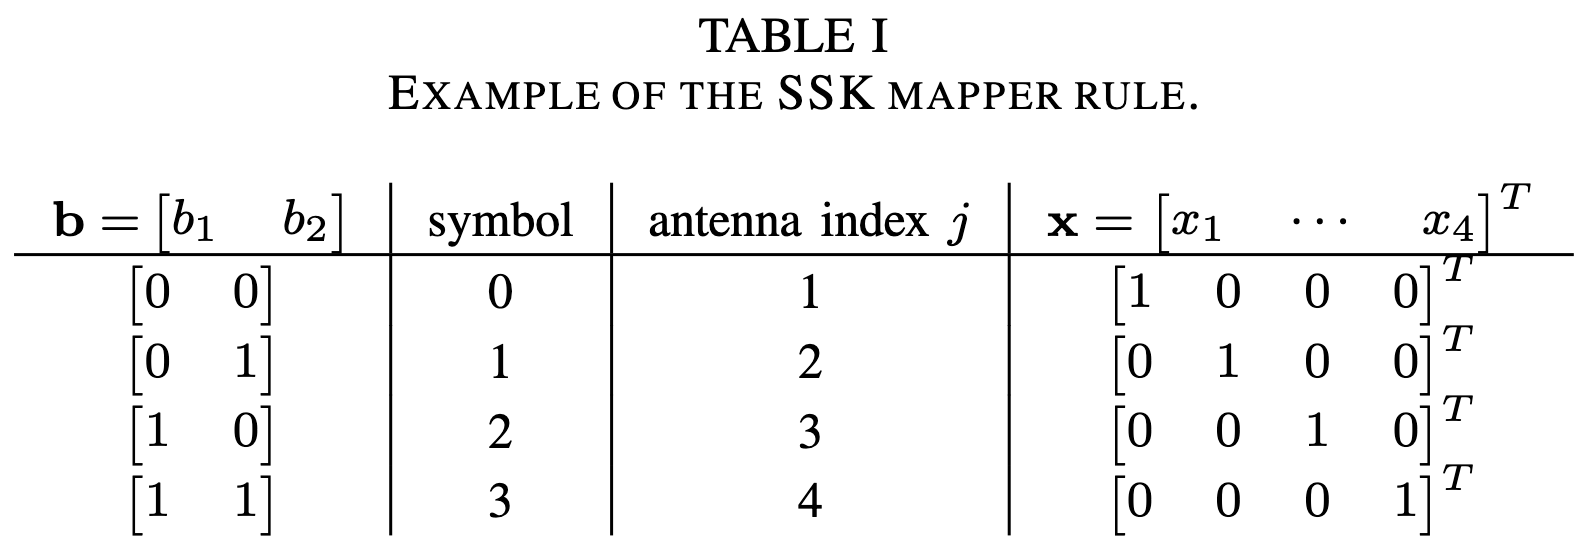
\includegraphics[width=\linewidth]{imgs/ssk_conversion_table.png}
  \caption{SSK conversion table [From \cite{5165332}]}
  \label{fig:ssk_conversion_table}
\end{figure}

\subsubsection{Direct Detection}
Given a channel gain matrix $\bm{B} \in \C^{KxK}$ and the input vector $x \in \C^K$ with only one element equal to $1$, the signal received is
\begin{equation}
  y = \bm{B}x + \sigma^2
\end{equation}
To understand the antenna index which sent the message, we need to find the column $b_j$ which is most similar to $y$.

\begin{equation}
  j = \argmax_j\ p_y (y | x_j, \bm{B}) = \argmin_j\ || y - b_j ||^2
  \label{eq:direct_detection}
\end{equation}

\subsubsection{Diagonalized Reflection Detection}
Following \cite{9328149}, for a reflected signal we have
\begin{equation}
  y = \bm{GPH}x + \sigma^2
\end{equation}
Given that $\bm{GPH}$ is a diagonal matrix and $x$ has only one element equal to $1$, the resulting vector $\bm{GPH}x$ will still be a vector with only one element non zero. Adding noise, to find the antenna index we search for the biggest value in the vector.

\begin{equation}
  j = \argmax_j\ y_j
  \label{eq:reflection_detection}
\end{equation}